\documentclass[usenames,dvipsnames,pdftex,unicode,hidelinks]{beamer}
  \usepackage{cmap}
  \usepackage[T2A]{fontenc}
  \usepackage[utf8]{inputenc}
  \usepackage[english,russian]{babel}
  \usepackage{wasysym}
  \usepackage{mathtext} % для кириллицы в формулах
    \DeclareSymbolFont{T2Aletters}{T2A}{cmr}{m}{it} % кириллица в формулах курсивом

  \usepackage{tikz}
    \usetikzlibrary{positioning,fit,backgrounds}
  \graphicspath{{../img/}{../../img/}}

  % Русификация definition
  \newtheorem{ru-def}{Определение}
  \renewenvironment{definition}{\begin{ru-def}}{\end{ru-def}}

  % Начало раздела с показом его заголовка на весь кадр
  \newcommand{\splashsection}[1]{
    \section{#1}
    \begin{frame}[plain]
      \begin{center}
        \LARGE #1
      \end{center}
    \end{frame}
  }
  \newcommand{\I}{\mathrm{I}} % Интенсивность

  % add frame number to footline
  \let\oldmacro\insertshorttitle
  \renewcommand*\insertshorttitle{
    \oldmacro\hfill
    \insertframenumber\,/\,\inserttotalframenumber
  }

  % hide navigation symbols
  \beamertemplatenavigationsymbolsempty

  \usetheme{Warsaw}
  \usecolortheme{seahorse}
  \usefonttheme{structurebold}

  \setbeamercovered{transparent}

  \newcommand{\muted}[1]{\textcolor{gray}{#1}}

  \newcommand{\vect}[1]{\vec{#1}} % единое выделение векторов (стрелкой)
  \newcommand{\matx}[1]{\mathbf{#1}} % единое выделение матриц (полужирным)
  \newcommand{\transposed}{\top} % единый знак транспонирования (U+22A4 down tack)
  \newcommand{\conj}[1]{#1^*} % единое обозначение комплексного сопряжения (черта сверху)
  \renewcommand{\le}{\leqslant} % <= с наклонной нижней перекладиной
  \renewcommand{\ge}{\geqslant} % >= с наклонной нижней перекладиной
  \renewcommand{\phi}{\varphi} % phi завитушкой

  \newcommand{\mathalert}[1]{
    \tikz[baseline]{
      \node [fill=red!30,anchor=base] {$ #1 $};
    }
  }

\title[Интерференция]{Интерференция}
\author[Иван Новиков]{
  Новиков Иван Александрович\texorpdfstring{
    \\
    \vspace{0.5cm}
    \small 1 курс магистратуры ФТФ,\\
           Физика / инф. пр. и сист.
  }{
    - КубГУ, ФТФ, 1 курс магистратуры
  }
}

\institute{Кубанский Государственный Университет}

\date{ \today }

\begin{document}
  
  % Local background must be enclosed by curly braces for grouping.
  {
    \usebackgroundtemplate{
      \newcounter{cntShader}
      \begin{tikzpicture}[show background rectangle, inner frame sep=2mm, background rectangle/.style={ draw=none }]
        \foreach \x in {-4, ..., 21} {
          \foreach \y in {-3, ..., 15} {
            \pgfmathsetcounter{cntShader}{ 500 / (abs(\x) + 1) / (abs(\y) + 1)}
            \shade[shading=radial,inner color = blue!\thecntShader] (\x*0.5, \y*0.5) circle (0.1);
          }
        }
      \end{tikzpicture}
    }
    \begin{frame}[plain]
      \titlepage
    \end{frame}
  }

  \begin{frame}{Понятие интерференции}
    \begin{definition}
      \alert{Интерференция} волн \muted{(от лат. inter - взаимно, между собой и ferio - ударяю, поражаю)}
      --- взаимное усиление или ослабление двух (или большего числа) волн при их наложении друг на
      друга при одновременном распространении в пространстве.

      \begin{flushright}
        --- Физическая энциклопедия
      \end{flushright}
    \end{definition}

    \uncover<2->{
      \begin{center}
        \begin{tikzpicture}[scale=2, transform shape]
          \node {\textrm{ $\I_{1+2} \neq \I_1 + \I_2 $ }};
        \end{tikzpicture}
      \end{center}
    }

    \begin{block}{}
      Обычно под интерференционным эффектом понимается \alert<2->{отличие} результирующей интенсивности
      волнового поля \alert<2->{от~суммы интенсивностей} исходных волн.
    \end{block}
  \end{frame}

  \begin{frame}{Наблюдается на любых волнах}
    \begin{itemize}
      \item<1> Акустические, радиоволны, волны на поверхности воды...
        \begin{center}
          \visible<1>{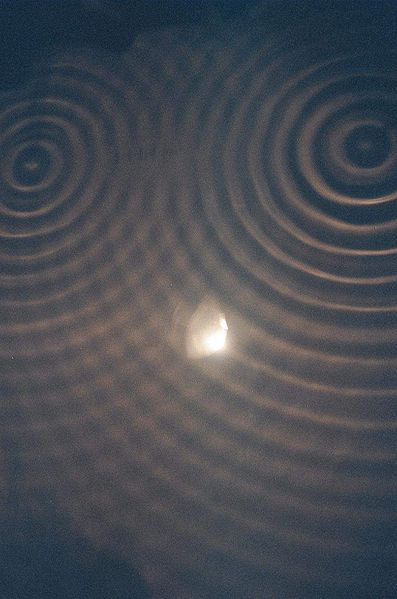
\includegraphics[width=0.3\textheight,angle=90]{water-interference}}
        \end{center}
      \item<2> ...но нагляднее всего на \alert{световых} волнах
        \begin{center}
          \visible<2>{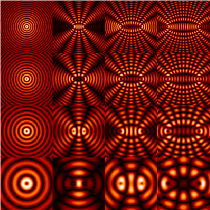
\includegraphics[height=0.4\textheight]{wavepanel}}
        \end{center}
    \end{itemize}
  \end{frame}

  \begin{frame}{Механизм интерференции}
    Проще всего понять на двух крайних случаях сложения волн:
    \vspace{5mm}
    \begin{enumerate}
      \item<1> Интерференционное усиление:
        \begin{tikzpicture}
          \draw[red, thick, smooth, domain=0:4.5, samples=50] plot (\x, {0.3*sin(8*\x r)});
          \node (plus) at (2, 0.5) {+};
          \draw[red, thick, smooth, domain=0:4.5, samples=50] plot (\x, {1 + 0.3*sin(8*\x r)});
          \node (equals) at (5, 0.5) {=};
          \draw[red, ultra thick, smooth, domain=5.5:9.8, samples=50] plot (\x, {0.5 + 0.6*sin(8*\x r)});
        \end{tikzpicture}
        --- если волны совпадают по фазе
        \vspace{5mm}
      \item<2> Интерференционное гашение:
        \begin{tikzpicture}
          \draw[red, thick, smooth, domain=0.4:4.9, samples=50] plot (\x, {0.3*sin( (8*\x + pi) r)});
          \node (plus) at (2, 0.5) {+};
          \draw[red, thick, smooth, domain=0:4.5, samples=50] plot (\x, {1 + 0.3*sin(8*\x r)});
          \node (equals) at (5, 0.5) {=};
          \draw[red, ultra thick, smooth, domain=5.5:9.8, samples=2] plot (\x, {0.5 + 0*\x}); % !!  samples = 2 - оптимизация для прямой!
        \end{tikzpicture}
        --- если одна волна отстаёт от другой на половину периода
    \end{enumerate}
  \end{frame}

  \begin{frame}{Математическое обоснование}

    \begin{itemize}[<+->]
      \item Свет~--- электромагнитная волна
      \item Рассмотрим плоскую электромагнитную волну, в ней напряжённость электрического поля
        \[
          \vect{E}(t, \vect{r}) = \vect{E}_0 \cdot e^{i(\omega t + (\vect{k}\cdot\vect{r}) + \phi)}
        \]
      \item Интенсивность определяется квадратом модуля напряжённости поля: $\I = |\vect{E}|^2 = E\cdot\conj{E}$
      \item При сложении двух таких волн поле: $\vect{E} = \vect{E}_1 + \vect{E}_2$ \\ \muted{(принцип суперпозиции)}
      \item Тогда интенсивность получаемой волны:
        \[
          \I = |\vect{E}_1 + \vect{E}_2|^2 = E_1^2 + E_2^2 + (\vect{E}_1\conj{\vect{E}_2} + \conj{\vect{E}_1}\vect{E}_2) =
        \]\[
          = \I_1 + \I_2 + \mathalert{2 \vect{E}_{01} \vect{E}_{02} \cdot \cos \left( (\vect{k}_1\cdot\vect{r}) -
            (\vect{k}_2\cdot\vect{r}) + \phi_1 - \phi_2 \right)}
        \]
    \end{itemize}
    
  \end{frame}

  \begin{frame}{Интерференционная картина}
    \begin{itemize}[<+->]
      \item Итак, интенсивность:
        \[
          \I = \I_1 + \I_2 + 2 (\vect{E}_{01} \cdot \vect{E}_{02}) \cdot \cos \left( (\vect{k}_1\cdot\vect{r}) -
               (\vect{k}_2\cdot\vect{r}) + \phi_1 - \phi_2 \right)
        \]
      \item В одномерном случае $\vect{r} = (x, 0, 0)$ и при сонаправленных поляризациях:
        \[
          \I = \I_1 + \I_2 + 2 \sqrt{I_1 I_2} \cdot \cos \left(
            \mathalert{(k_{1_x} - k_{2_x}) \cdot x}
          + \phi_1 - \phi_2 \right)
        \]
      \item Возникают чередующиеся полосы с шагом $h=\frac{2\pi}{k_{1_x}-k_{2_x}}$:
        \begin{center}
          \begin{tikzpicture}
            \foreach \x in {1, ..., 20}
            \shade[left color=white, right color=white, middle color=red!75] (0.2*\x, 0) rectangle (0.2 + 0.2*\x, 2);
          \end{tikzpicture}
        \end{center}
    \end{itemize}
  \end{frame}

  \begin{frame}{Случай разных частот}
    \begin{itemize}[<+->]
      \item Если $\omega_1 \neq \omega_2$:
        \[
          \vect{E}_1=\vect{E}_{01}\cdot e^{i({\omega}_{1}t + (\vec{k}_1 \cdot \vec{r}_1) + {\phi}_1)},
          \hspace{5mm}
          \vect{E}_2=\vect{E}_{02}\cdot e^{i({\omega}_{2}t + (\vec{k}_2 \cdot \vec{r}_2) + {\phi}_2)}
        \]
      \item Интенсивность рассматриваем как усреднённый по времени квадрат амплитуды:
        \[
          \I = {<{E}}^2{>}_\tau
        \]
      \item Тогда после усреднения по времени выражения для $\I$:
        { \small
        \[
          \I = \I_1 + \I_2 + 2(\vect{E}_{01} \cdot \vect{E}_{02}) \cos \left(
            \mathalert{\Delta\omega (t_0+\frac{\tau}{2})} + \Delta \vect{k}\vect{r} + \Delta\phi
          \right) \mathalert{ \operatorname{sinc}(\frac{\Delta\omega\tau}{2}) }
        \]
        }
    \end{itemize}
    
  \end{frame}

  \begin{frame}{Условия возникновения интерференции}

    { \small
    \[
      \boxed{
        \I = \I_1 + \I_2 + 2(\vect{E}_{01} \cdot \vect{E}_{02}) \cdot\cos \left( \Delta\omega (t_0+\frac{\tau}{2})+\Delta
        \vect{k}\vect{r}+\Delta\phi \right) \cdot \operatorname{sinc}(\frac{\Delta\omega\tau}{2})
      }
    \]
    }
    \begin{enumerate}[<+->]
      \item Поляризации \emph{не} должны быть перпендикулярны\\
        \muted{(иначе $(\vect{E}_{01} \cdot \vect{E}_{02}) = 0$)}
        \vspace{5mm}
      \item Частоты не должны существенно отличаться\\
        \muted{(иначе $\operatorname{sinc}(\frac{\Delta\omega\tau}{2}) \approx 0$)}
        \vspace{5mm}
      \item Волны должны быть \emph{когерентны}\\
        \muted{(иначе $\Delta\phi$ меняется случайным образом и теряется при усреднении)}
    \end{enumerate}

  \end{frame}

  \begin{frame}{Наблюдение интерференции: опыт Юнга}
    \begin{center}
      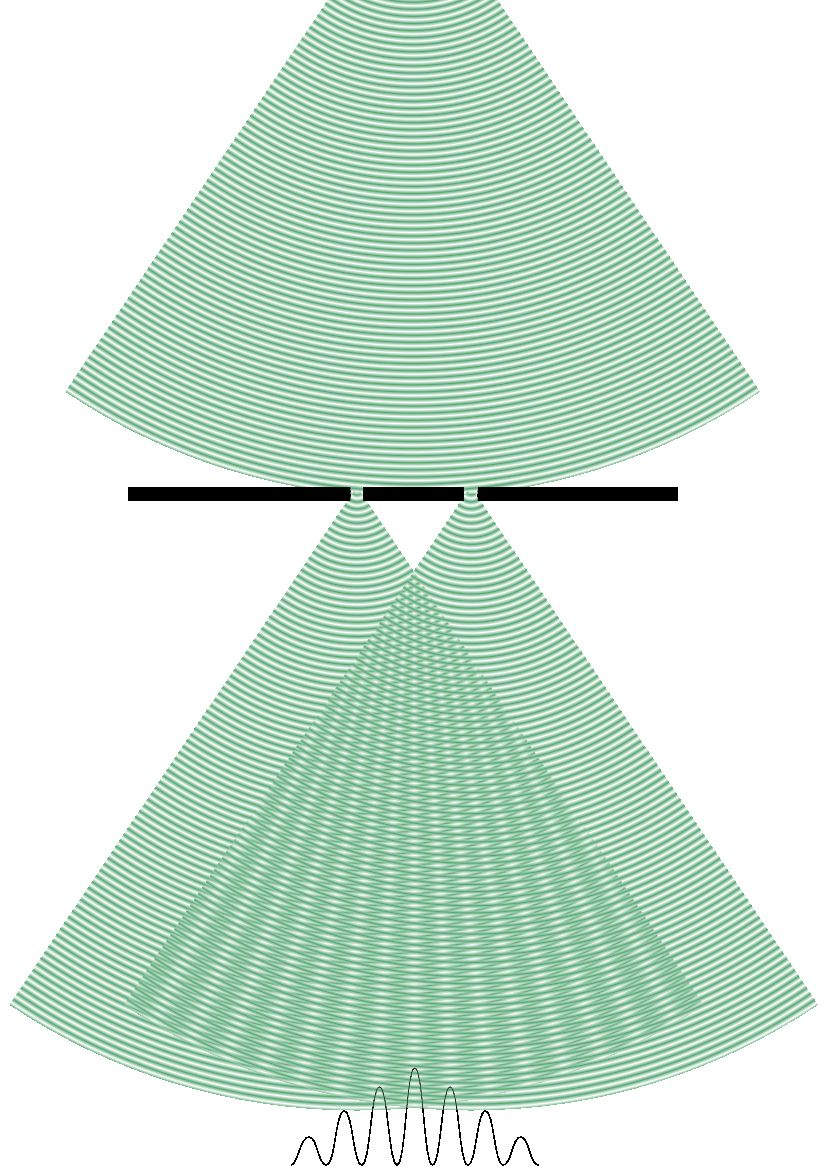
\includegraphics[height=0.75\textheight]{young}
    \end{center}
  \end{frame}

  \begin{frame}{Наблюдение интерференции: кольца Ньютона}
    \begin{center}
      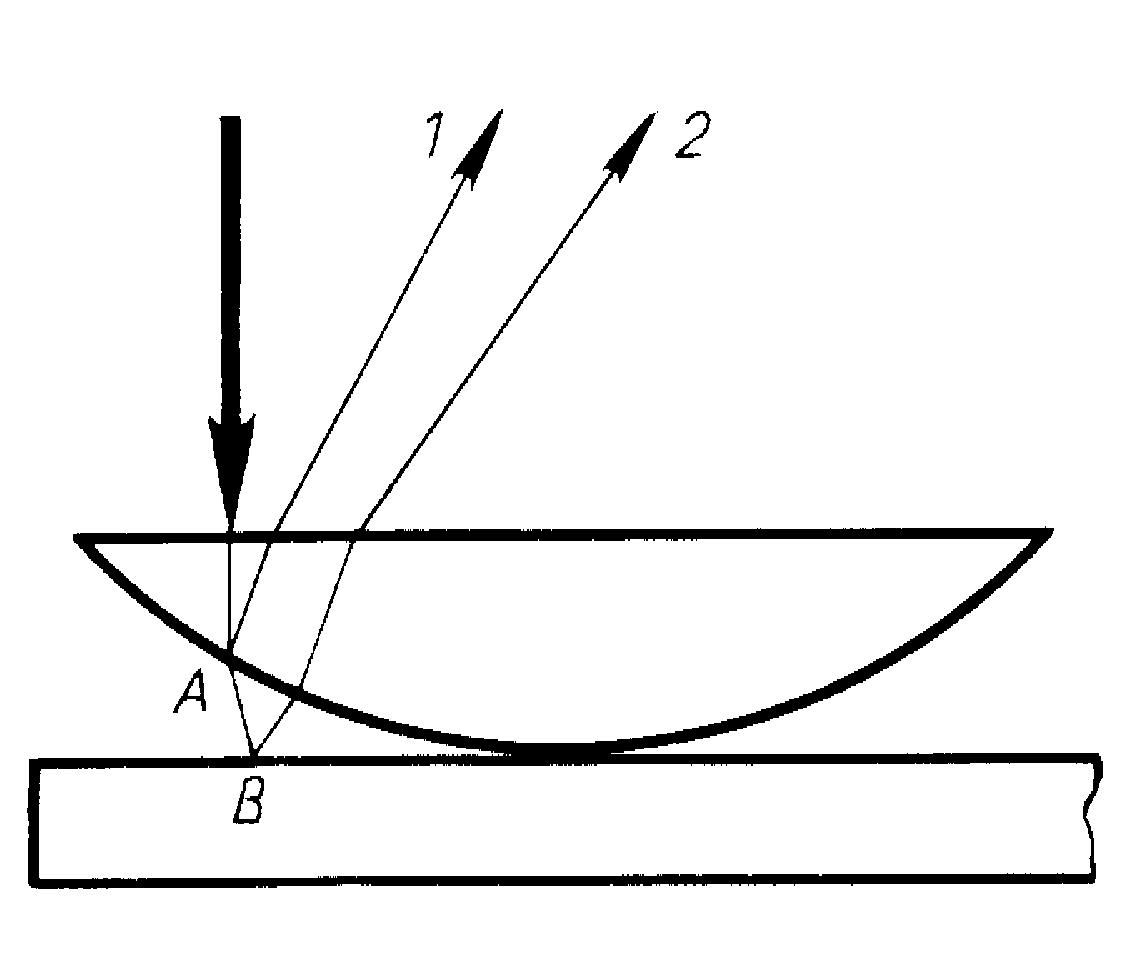
\includegraphics[height=0.5\textheight]{newton-rings-scheme}
      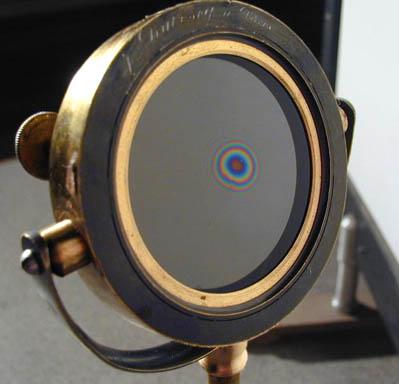
\includegraphics[height=0.5\textheight]{newton-rings}
    \end{center}
  \end{frame}

  \begin{frame}{Наблюдение интерференции: тонкие плёнки}
    \begin{center}
      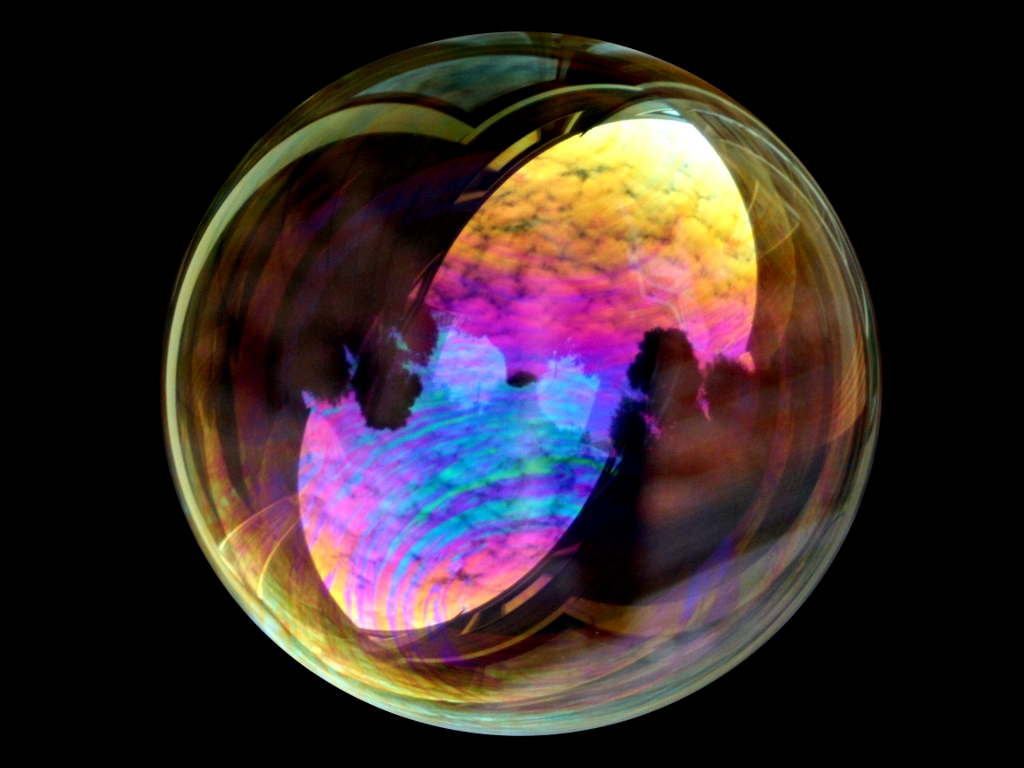
\includegraphics[height=0.6\textheight]{bubble}
      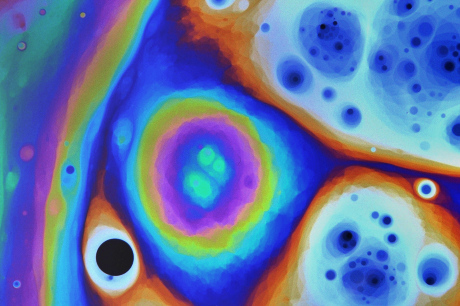
\includegraphics[width=0.6\textheight,angle=90]{thin-film}
    \end{center}
  \end{frame}

  \begin{frame}{Применения интерференции:\\ Определение показателя преломления}
    \begin{center}
      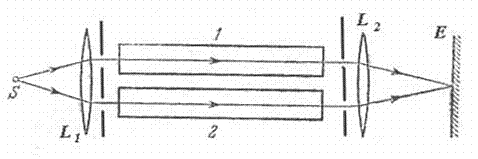
\includegraphics[width=0.75\textwidth]{n}
    \end{center}
    \begin{block}{}
      Оптической разности хода лучей соответствует смещение
      интерференционной картины на некоторое число полос $N_{int}$ относительно направления
      центрального максимума. Значение показателя преломления исследуемого вещества может быть найдено по формуле:
      $
        n = 1 + N_{int} \frac{\lambda}{l}
      $
    \end{block}
  \end{frame}

  \begin{frame}{Применения интерференции:\\ Определение размеров звёзд}
    \begin{center}
      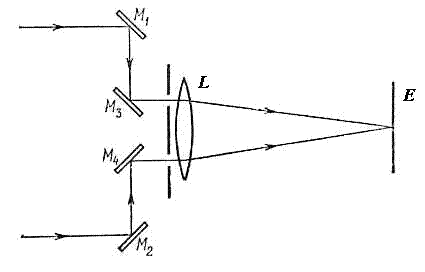
\includegraphics[height=0.5\textheight]{star-size}
      \begin{block}{}
        Наблюдение интерференционной картины, создаваемой двумя щелями, расстояние между которыми
        равно $d$ и освещаемые светом длиной волны $\lambda$, возможно, если $d < 2 \rho_c$, где
        $\rho_c$~--- радиус пространственной когерентности источника света.
      \end{block}
    \end{center}
  \end{frame}

  \begin{frame}{Применения интерференции:\\ просветление оптики}
    \begin{center}
      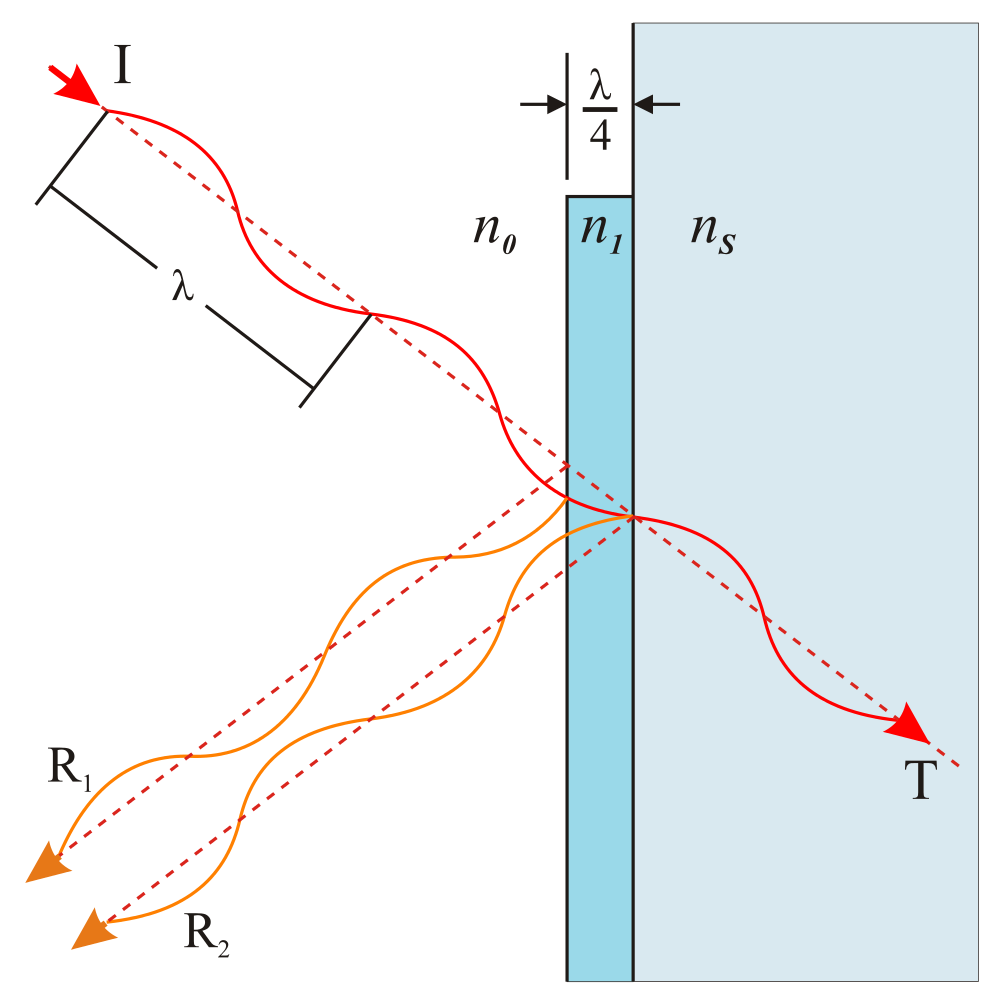
\includegraphics[height=0.5\textheight]{antireflection}
      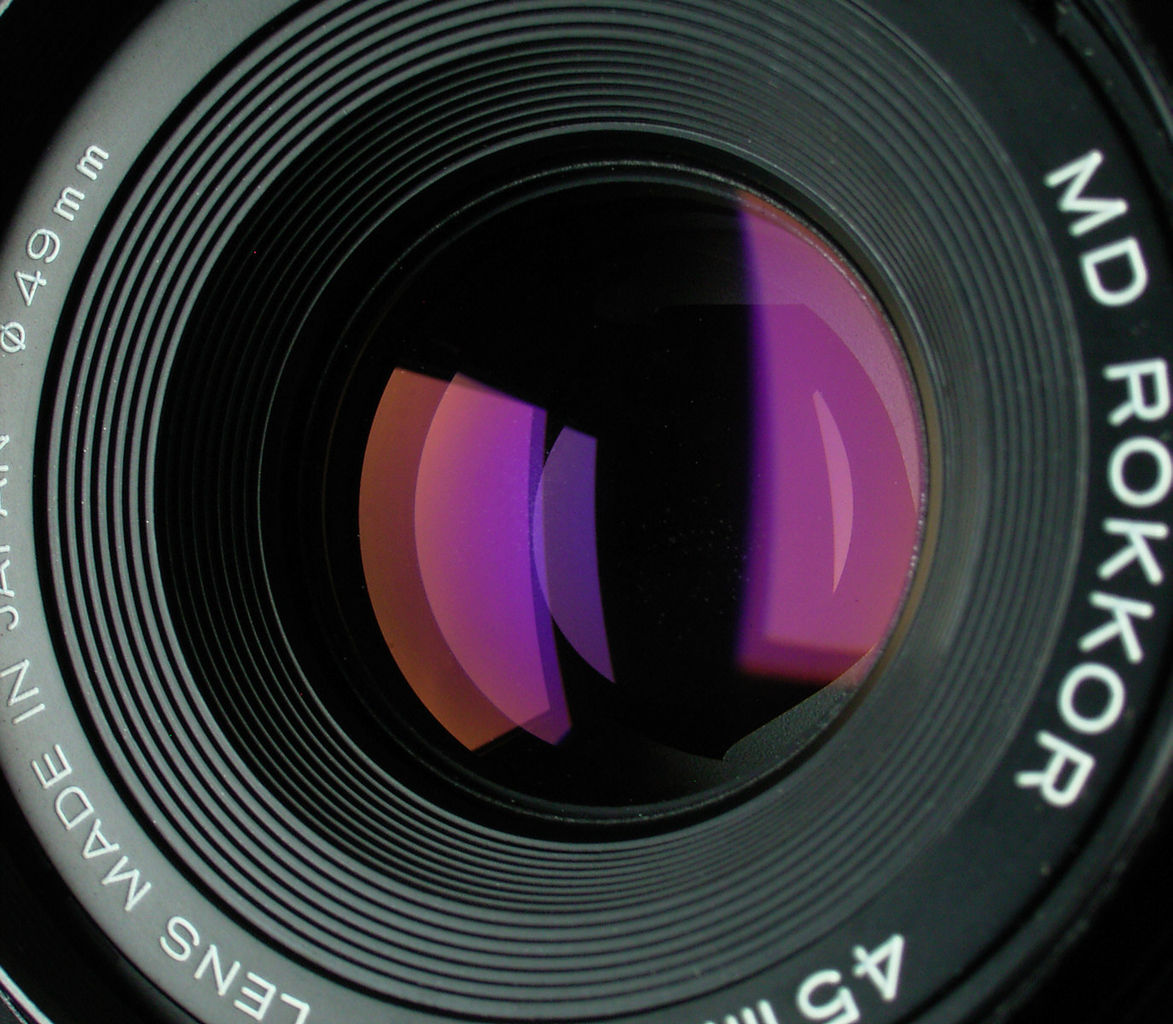
\includegraphics[height=0.5\textheight]{lens}
      \begin{block}{}
        Интерференционном гашение волны, отраженной от внешней поверхности покрытия, волной отражённой от внутренней.
        Амплитуды волн должны быть равны, а фазы отличаться на $\pi$.
      \end{block}
    \end{center}
  \end{frame}

  \begin{frame}{Применения интерференции:\\ Голография}
    \begin{center}
      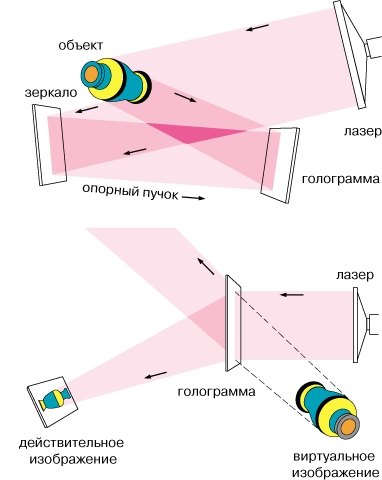
\includegraphics[height=0.6\textheight]{holography}
      \hspace{5mm}
      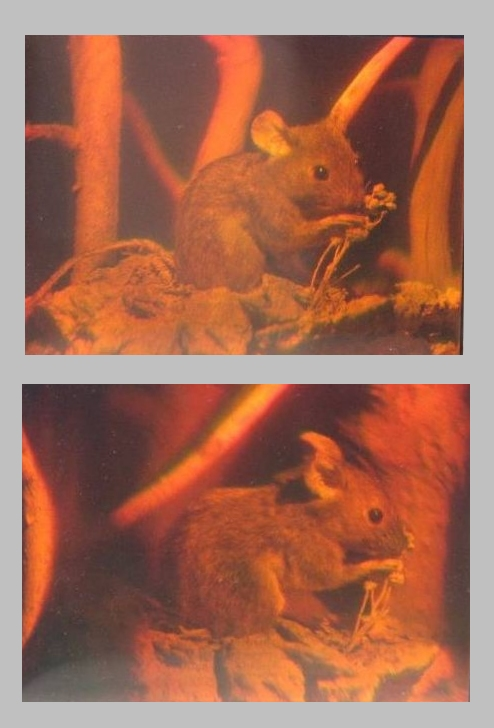
\includegraphics[height=0.6\textheight]{holomouse}
      \begin{block}{}
        Запись интерференционной картины: регистрация не только амплитуды волнового поля, но и фазы
      \end{block}
    \end{center}
  \end{frame}

  \begin{frame}{Заключение}
    \begin{block}{Вывод}
      Интерференция~--- одно из важнейших оптических явлений, являющееся составной частью других
      явлений (например, дифракции) и имеющее множество применений в современной науке и технике.
    \end{block}
  \end{frame}

  \begin{frame}[plain]
    \begin{center}
      { \Huge Спасибо за внимание! }

      \vspace{1cm}

      Иван Новиков\\
      \url{http://about.me/moonlighter}\\
      \href{mailto:nia.afti@gmail.com}{\nolinkurl{nia.afti@gmail.com} }
      
    \end{center}
  \end{frame}

\end{document}

